\section*{Methodology}
\addcontentsline{toc}{section}{Methodology}

\phantomsection
\subsection*{Design Development Logic}
\addcontentsline{toc}{subsection}{Design Development Logic}

\begin{figure}[H]
\centering
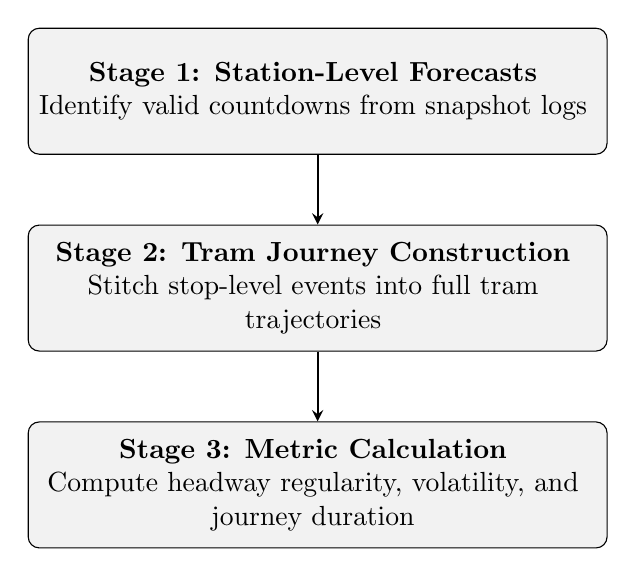
\begin{tikzpicture}[node distance=2.5cm]

\tikzstyle{process} = [rectangle, rounded corners, minimum width=5.5cm, minimum height=1.6cm, text centered, draw=black, fill=gray!10, align=center]
\tikzstyle{arrow} = [thick,->,>=stealth]

\node (stage1) [process] {
    \begin{minipage}{7cm}
    \centering
    \textbf{Stage 1: Station-Level Forecasts}\\
    Identify valid countdowns from snapshot logs
    \end{minipage}
};
\node (stage2) [process, below of=stage1] {
    \begin{minipage}{7cm}
    \centering
    \textbf{Stage 2: Tram Journey Construction}\\
    Stitch stop-level events into full tram trajectories
    \end{minipage}
};
\node (stage3) [process, below of=stage2] {
    \begin{minipage}{7cm}
    \centering
    \textbf{Stage 3: Metric Calculation}\\
    Compute headway regularity, volatility, and journey duration
    \end{minipage}
};

\draw [arrow] (stage1) -- (stage2);
\draw [arrow] (stage2) -- (stage3);

\end{tikzpicture}
\caption{Three-stage Pipeline}
\label{fig:processing-flowchart}
\end{figure}

    Early attempts to construct LUAS tram journeys directly from raw forecasts aimed to generate both single-stop arrivals and full-route forecasts in one processing step. However, this approach quickly proved unmanageable, due to excessive aggregation, duplicate assignments, and ambiguous mappings, which compromised data clarity and reliability. These issues were especially pronounced around city centre stations, where high service frequency, shared-route stops, and inconsistent directional inference complicated accurate reconstruction. In response to these shortcomings, the construction process was restructured into a multi-stage plan to improve reproducibility and maintain control while ensuring the accurate building of services. A rule-based approach was selected over machine learning or simulation-based alternatives to ensure transparency, interpretability, and full control over how forecasts were translated into operational journeys, as the scale and intricacy of real-world transit activity risk being lost or oversimplified in more abstracted modelling methods.

    Stage one focused on grouping raw forecast logs into coherent station-level tram segments. Stage two then constructed full tram trips by assembling these segments according to predefined stop templates, ensuring directionally valid and physically plausible routes. Stage three applied analytic transformations to the stitched journeys to allow for the computation and visualisation of the performance metrics. This process was refined through staged development, with initial prototypes tested on a single month to validate forecast chunking and route-matching logic before being scaled across the full dataset and pandemic phases. The resulting modular pipeline was designed to handle the large data, concurrent operations, and potential irregularities, enabling a systematic review of service reliability.



\phantomsection
\subsection*{Stage 1: Building Station-Level Forecasts}
\addcontentsline{toc}{subsection}{Stage 1: Building Station-Level Forecasts}

    The first stage of journey reconstruction involved identifying coherent sequences of predicted tram arrivals at individual LUAS stations. Because the dataset contained no unique vehicle identifiers, it was necessary to infer per-tram behaviour through the analysis of arrival prediction evolution. To achieve this, raw forecast logs were first grouped by \texttt{Line}, \texttt{Destination}, \texttt{Station}, and \texttt{ServiceDay}, and then sorted chronologically by the forecast timestamp (\texttt{DateTime}). Each log captured a forecasted number of minutes until a tram’s expected arrival at a station, recorded at roughly two-minute intervals; over time, these snapshots formed countdown sequences that tracked the predicted approach of a tram toward a stop. The function \texttt{stitch\_forecasts\_by\_station()} was developed to extract these sequences by scanning grouped logs for patterns that resembled realistic tram approaches. This process transformed disaggregated forecasts into discrete records, referred to as \texttt{StationJourneys}, each representing the inferred movement of a single tram arrival at a specified station. To isolate valid \texttt{StationJourneys}, the function applied four rule-based constraints: temporal continuity, countdown progression, sequence integrity, and minimum length. Each constraint addressed a key challenge in distinguishing real tram approaches from noise, logging anomalies, or overlapping vehicle forecasts, an essential step in high-frequency urban segments.

    Temporal continuity ensured that logs within a sequence were chronologically valid and associated with the same tram. To do this, entries were only linked if the time difference between consecutive logs was between 0 and 8 minutes. The upper limit prevented the erroneous merging of two separate trams that may have shared a destination and direction but were too far apart in time to plausibly belong to a single trip. The lower limit filtered out redundant duplicates, often caused by AVLS system miscalculations, latency-induced re-logging, or feed errors that recorded multiple timestamps within the same minute. Without this constraint, journeys could be artificially extended or misidentified, particularly in central segments where multiple trams in the same direction may appear within short intervals (peak periods). Along with this, the countdown progression leveraged the expectation that a tram approaching a stop should show a generally decreasing arrival time. Since forecasts were sampled every two minutes, an uninterrupted approach would typically show a two-minute drop between consecutive logs. However, AVLS are prone to short-term prediction noise due to signal delays, recalibration, or passenger boarding variation. To account for this, the function was designed to allow modest fluctuations: up to 2 minutes early (-2) or up to 5 minutes late (+5) between logs. The lower bound reflects a realistic allowance for minor system corrections, such as a tram arriving slightly ahead of forecast. The upper bound was selected based on exploratory testing, which showed that increases of more than 5 minutes were rare and often reflected a new tram entering the feed. These thresholds preserved the expectation of a steady countdown while accommodating real-world inconsistencies, ensuring only credible sequences were retained.

    Sequence integrity maintained logical structure by filtering out errors that could distort the inferred journeys. Repeated timestamps were removed to avoid inflating trip length through duplicated entries. Additionally, a reset condition was implemented to split sequences when a tram appeared to have arrived and was then followed by a new forecast. Specifically, if a log within a sequence showed a minimum prediction of less than or equal to 1 minute, and the following log showed an increase of 3 or more minutes, the sequence was cut at that point, and a new sequence was initiated. This logic handled common edge cases where a tram disappeared from the prediction feed and was rapidly replaced by the next approaching service, frequently seen in high-traffic segments. To further enforce sequence validity, a minimum forecast length ensured each retained log reflected a meaningful observation of tram movement. Sequences were required to contain at least five forecast entries to qualify as valid \texttt{StationJourneys}. This threshold was chosen to balance inclusivity and rigour: short enough to allow for partial journeys or low-frequency periods, but long enough to avoid retaining spurious or fragmentary prediction chains. Including too-short sequences risked misinterpreting random forecast noise as legitimate vehicle movement, which would undermine later network-level stitching.

    Together, these constraints enabled the transformation of raw, forecast data into structured station-level units representing plausible tram arrivals. Although no direct arrival flag exists, the final entry in each sequence is treated as a presumed arrival, inferred through countdown progression and the subsequent disappearance or reset of predictions in the forecast feed. With over 160 million records processed into coherent StationJourney segments, each tagged with a unique StationJourneyID, these sequences formed the foundational building blocks for all later stages of full-line reconstruction. Although the absence of vehicle-level IDs limited exact recreation, this rule-based logic produced reproducible sequences robust enough to support system-level reliability analysis. A sample output of a complete StationJourney is shown below (Figure~\ref{fig:station-level}), illustrating how a forecast countdown is linked from its initial appearance to the presumed arrival.

\begin{figure}[H]
  \centering
  \includegraphics[width=0.6\textwidth]{figures/paper_figures/station_level.png}
  \caption{Station-Level Forecast Segment Example}
  \label{fig:station-level}
\end{figure}

\phantomsection
\subsection*{Stage 2: Constructing Tram Journeys}
\addcontentsline{toc}{subsection}{Stage 2: Constructing Tram Journeys}

    The second stage of this study linked the previously stitched station-level segments into continuous, directionally valid journeys. This process relied on spatial and temporal alignment using predefined stop dictionaries, which served as structural references for identifying plausible combinations of \texttt{StationJourneysIDs} to represent a continuous tram journey. As these templates mirrored the physical order of LUAS stops by line and direction, a consistent matching process without reliance on operator or schedule assumptions was made possible. To implement this process, the \texttt{build\_clean\_tram\_journeys()} function first enriched the station-level logs with an \texttt{EstimatedArrival} variable, calculated by adding the predicted \texttt{Minutes} value to the log’s original timestamp (\texttt{DateTime}). This addition placed all forecasts on a uniform timeline of expected arrivals rather than forecast issuance, enabling a cleaner temporal comparison between stops. Additionally, the \texttt{ServiceDay} field was extracted to restrict stitching to individual operational days and prevent cross-day contamination.

    A lookup table (\texttt{sjid\_info}) was then constructed, containing each \texttt{Station\allowbreak Journey\allowbreak ID}’s station name, direction, estimated arrival time, and service day. This structure supported efficient iterative scanning of potential matches across possible segment combinations during the stitching process. Construction began by identifying a segment corresponding to the first stop in a given template. From this anchor, the function advanced sequentially through the stop order, attempting to append additional segments that matched both the expected stop and direction. To qualify, a candidate’s estimated arrival time had to fall within six minutes of the preceding segment. This temporal threshold approximated the realistic progression of travel times through the LUAS network, tolerating minor timing variations while minimising the risk of linking unrelated vehicles. Although not a strict headway value, the six-minute window served as a practical cutoff for inferring continuity, particularly in areas where tram forecasts often overlap.

    The function allowed for a maximum of one missing stop, improving resilience against forecast gaps or partial sequences and addressing common edge cases where forecasts were truncated or dropped near termini due to AVLS inconsistencies. However, all retained journeys were required to contain at least six matched stops to qualify for inclusion; this threshold ensured that even reduced services reflected genuine vehicle movement. A stricter filter, requiring 15 stops, was later applied during metrics calculation to isolate near-complete journeys suitable for analysis. Furthermore, to prevent duplication and ensure segment uniqueness, each \texttt{StationJourneyID} was assigned to only one \texttt{TramJourney}. Once a segment was successfully matched, it was flagged as used and excluded from subsequent iterations. This safeguard was important in central LUAS segments with shared tracks and overlapping directions, where sequence ambiguity was more likely. Upon completion, each journey was assigned a unique \texttt{TramJourneyID}, constructed from its origin, destination, and service day, with an incremental counter (\texttt{BRO\_SAN03\_2021\_06\_14}), enabling consistent referencing in downstream analysis.

    Although the absence of explicit tram vehicle identifiers limited the ability to track individual units, this approach produced repeatable and interpretable approximations of real-world tram movements. By integrating structured stop templates, estimated arrivals, and conservative temporal thresholds, fragmented station-level logs were reconstructed into coherent, plausible journeys. While some uncertainty remains due to prediction gaps or AVLS anomalies, the resulting dataset is robust enough to support comprehensive reliability evaluation in the next stage.

\phantomsection
\subsection*{Stage 3: Computing Reliability Metrics}
\addcontentsline{toc}{subsection}{Stage 3: Computing Reliability Metrics}

    With tram journeys reconstructed and grouped, the resulting records formed the basis for computing the three key transit metrics: headway regularity, travel time volatility, and journey duration. Due to the uneven durations of the phases, these were averaged and further disaggregated by time of day to capture fluctuations. The \texttt{generate\allowbreak\_final\allowbreak\_segments()} function transformed each \texttt{TramJourneyID} into a sequence of inter-station segments by retaining only the final forecast log for each \texttt{StationJourneyID}, representing the final predicted arrival of a tram at each stop. These arrival logs were kept in stop template order, and station pairs (each log’s Current Station to its Next Station) were linked to calculate \texttt{TravelTimeMinutes}, the inferred duration between two consecutive stops. To illustrate the resulting final segments, Figure~\ref{fig:arrival_journey} presents a single complete tram journey.

\begin{figure}[H]
  \centering
  \includegraphics[width=0.6\textwidth]{figures/paper_figures/arrival_journey.png}
  \caption{Example of an Arrival Journey}
  \label{fig:arrival_journey}
\end{figure}

    Headway regularity was used to assess the consistency of tram arrivals during stages of high demand; these were calculated as the time intervals between two consecutive trams at the same stop, grouped by line and direction to account for overlapping services along shared-direction tracks. For each stop, arrival times were sorted chronologically, and the time difference between successive trams was saved as \texttt{HeadwayMinutes}. These values were then binned into two peak periods, Morning (06:00 to 10:00) and Evening (15:00 to 19:00), to isolate intervals of high passenger demand where service regularity was most critical. To reduce the influence of outlier values caused by disruptions or noise, Interquartile Range (IQR) filtering was applied. The resulting \texttt{AvgHeadwayMinutes} provided a measure of how evenly spaced trams were at each stop, helping to identify locations with irregular service frequency or potential gaps. Inconsistent headways can indicate a need for increased vehicle deployment or operational adjustments to improve line-level reliability and passenger experience.

    Travel time volatility (TTV) was used to quantify the consistency of travel durations between consecutive stops. For each inter-stop segment (Stop → NextStop), the standard deviation of \texttt{TravelTimeMinutes} was calculated and grouped by hour of day. These hourly TTV values were then averaged across the broader periods (Morning, Midday, Evening, and Night) and grouped by line and direction; this breakdown enabled the identification of when and where tram movement was most variable. High volatility values indicated operational instability or external disruptions that affected the predictability of arrival times. By highlighting segments with greater variability, TTV helped reveal structural inefficiencies in the network. This metric can support targeted interventions such as timetable refinements, signal prioritisation, or infrastructure improvements to improve the regularity and predictability of tram movement across specific corridors.

    Journey duration provided a baseline for evaluating overall service efficiency, measuring the total time taken by each reconstructed tram journey from start to end. Rather than using the difference between the first and last arrival timestamps, duration was computed by summing the \texttt{TravelTimeMinutes} values for all inter-stop segments within each \texttt{TramJourneyID}. This method accounted for inconsistent spacing or incomplete countdowns and offered a more reliable reflection of real movement, particularly where arrival predictions were irregular or truncated before reaching zero. Each journey was categorised by its starting hour into time-of-day periods to enable comparative analysis across demand windows. IQR filtering was again applied to remove extreme durations, producing a refined dataset representative of typical service conditions. Trends in journey duration across phases and directions offered insights into broader operations and allowed planners to detect stretches requiring schedule adjustments, address systemic slowdowns, or further look into congestion-prone areas.

    Together, these three measurements offered a comprehensive framework for assessing LUAS service over time, enabling the identification of both spatial and temporal inconsistencies in delivery. The structured outputs supported comparative analysis of operative adaptations to evolving conditions across pandemic phases. Additionally, by incorporating time-of-day breakdowns within each phase, the analysis can capture intra-day variability in performance. These measures ensured that the reconstructed dataset could support robust, reproducible evaluations of network reliability, grounded in established transit research methodologies and responsive to real-world operational dynamics.

